\documentclass{llncs}
\usepackage[utf8x]{inputenc}
\usepackage{url}
\usepackage{tikz}
\usepackage{graphicx}
\usepackage{amsmath,amssymb,algorithm2e}
\usepackage{listings,color}
\usepackage{xspace}
\usepackage{algorithmic}

\parindent 0em
\parskip 0.5em

\title{Breaking An Identity-Based Encryption Scheme based on DHIES}

\author{Martin R. Albrecht\inst{1} \and Kenneth G. Paterson\inst{2}\thanks{This
author supported by an EPSRC Leadership Fellowship, EP/H005455/1.}}

\institute{INRIA, Paris-Rocquencourt Center, SALSA Project
UPMC Univ Paris 06, UMR 7606, LIP6, F-75005, Paris, France
CNRS, UMR 7606, LIP6, F-75005, Paris, France
\and Information Security Group, Royal Holloway, University of London.}

\newcommand{\heading}[1]{{\vspace{6pt}\noindent\sc{#1.}}}

\newcommand{\ring}[1]{\mathbb{#1}}
\newcommand{\Z}{\ensuremath{\ring{Z}}\xspace}
\newcommand{\FX}{\ensuremath{\Z_q[x_0,\dots,x_{n-1}]}\xspace}
\newcommand{\sys}{\ensuremath{f_0,\dots,f_{m-1}}\xspace}
\newcommand{\ideal}[1]{\ensuremath{\langle #1 \rangle}\xspace}

\newcommand{\LM}{\ensuremath{\textsc{LM}}\xspace}
\newcommand{\LC}{\ensuremath{\textsc{LC}}\xspace}
\newcommand{\LT}{\ensuremath{\textsc{LT}}\xspace}
\newcommand{\LCM}{\ensuremath{\textsc{LCM}}\xspace}
\newcommand{\GCD}{\ensuremath{\textsc{GCD}}\xspace}
\newcommand{\Mac}[1]{\ensuremath{\mathcal{M}^{acaulay}_{#1}}}

\newcommand{\e}{\ensuremath{\mathbf{e}}\xspace}

\newcommand{\ord}[1]{\ensuremath{\mathcal{O}\!\left(#1\right)}}

\newcommand{\malbnote}[1]{{\color{red}\textbf{malb}: {\it #1}}}
\newcommand{\kpnote}[1]{\textbf{kp: {\it #1}}}

\newcommand{\SKE}{\ensuremath{\mathsf{SKE}}\xspace}
\newcommand{\PKE}{\ensuremath{\mathsf{PKE}}\xspace}

\newcommand{\Gen}{\mathsf{Gen}}
\newcommand{\Enc}{\mathsf{Enc}}
\newcommand{\Eval}{\mathsf{Eval}}
\newcommand{\Dec}{\mathsf{Dec}}
\newcommand{\SK}{\mathsf{SK}}
\newcommand{\PK}{\mathsf{PK}}
\newcommand{\msg}{\mathsf{m}}
\newcommand{\cph}{\mathsf{c}}
\newcommand{\key}{\mathsf{k}}
\newcommand{\MsgSp}{\mathsf{MsgSp}}
\newcommand{\RndSp}{\mathsf{RndSp}}
\newcommand{\ReRand}{\mathsf{ReRand}}
\newcommand{\Circt}{\mathcal{C}}

\newcommand{\A}{\ensuremath{\mathcal{A}}\xspace}
\newcommand{\B}{\ensuremath{\mathcal{B}}\xspace}
\newcommand{\G}{\ensuremath{\mathcal{G}}\xspace}
\newcommand{\IND}{\mathsf{IND}}
\newcommand{\ind}{\mathsf{ind}}
\newcommand{\CPA}{\mathsf{CPA}}
\newcommand{\cpa}{\mathsf{cpa}}
\newcommand{\KDM}{\mathsf{KDM}}
\newcommand{\kdm}{\mathsf{kdm}}
\newcommand{\Initialize}{\mathbf{Initialize}}
\newcommand{\Finalize}{\mathbf{Finalize}}
\newcommand{\LR}{\mathbf{Left\mbox{-}Right}}
\newcommand{\Encrypt}{\mathbf{Encrypt}}
\newcommand{\sample}{{\;{{\leftarrow}_\$}\;}}
\newcommand{\Adv}{\mathbf{Adv}}
\newcommand{\true}{\mathsf{T}}
\newcommand{\false}{\mathsf{F}}

\lstdefinelanguage{Sage}[]{Python}
{morekeywords={True,False,sage},
sensitive=true}

\lstset{frame=single,
          showtabs=False,
          showspaces=False,
          showstringspaces=False,
          keywordstyle={\bfseries},
          language=Sage}

\begin{document}

\maketitle

\begin{abstract}
We present collusion attacks against a recently proposed IBE scheme of Chen {\em et al.} from ASIACCS 2010. The attacks recover the master secret key of the scheme and thereby invalidate the existing security analysis of this scheme. The attacks are flexible, allowing, for example, the amount of computation needed to be traded-off against the size of the collusion.

\vspace{0.1cm}

\noindent {\bf Keywords:} identity-based encryption; cryptanalysis; Gr\"{o}bner bases.
\end{abstract}

\section{Introduction}

The search for Identity-Based Encryption (IBE) schemes having efficient algorithms and proven security has resulted in many proposals for schemes. A recent proposal, due to Chen {\em et al.} \cite{CCGHC10}, has very efficient encryption and decryption and claims to have security based on the security of the DHIES public key encryption scheme. In this paper, we present collusion attacks against the scheme of \cite{CCGHC10} which recover the Trusted Authority's master secret key. These attacks apply even in the weak IBE security model used in \cite{CCGHC10} and thus completely invalidate the security claims made in \cite[Theorem 3.1]{CCGHC10}, the main security result in that paper. We explain where the security analysis in \cite{CCGHC10} is deficient.

However, it seems that the authors of \cite{CCGHC10} were already aware of the possibility of collusion attacks against their scheme and set the scheme parameters with the intention of making such attacks inefficient (see Section 3.1 of \cite{CCGHC10}). We show that their setting of parameters is also flawed by exhibiting a family of efficient collusion attacks against the scheme which applies for their concrete choice of parameters. In fact, our attacks allow the various attack parameters to be traded off against one another -- such as the number of private keys needed (the size of the collusion), and the amount of computation needed. For example, we exhibit a master key recovery attack against the concrete scheme of \cite{CCGHC10} that requires a collusion of $2^{13}$ parties, $2^{43.3}$ evaluations of a hash function and $2^{30}$ field operations.
 
In \cite{susilo-baek:asiaccs2011}, Susilo and Baek also present an attack against the scheme of \cite{CCGHC10}. We stress that our work was done independently of and in parallel to \cite{susilo-baek:asiaccs2011}. The attack in \cite{susilo-baek:asiaccs2011} is an application of the observation in Section 3.1 of \cite{CCGHC10} using more precise complexity results than the authors of the original scheme. As with our attacks, this invalidates the security claims made in \cite{CCGHC10}. However, our attacks are considerably more flexible, much more efficient than the attack in \cite{susilo-baek:asiaccs2011} and exploit more structure of the particular construction proposed in \cite{CCGHC10}. Moreover, we provide concrete attack costs for the parameters proposed in \cite{CCGHC10} (something that was omitted in \cite{susilo-baek:asiaccs2011}), we highlight the flaw in the security proof given in \cite{CCGHC10}, and we show that there is a design flaw in the construction of private keys in the scheme which enables attacks beyond straight-forward system solving. Finally, we note that \cite{susilo-baek:asiaccs2011} repeats some of the wrong claims made in \cite{CCGHC10} about the complexity of Gr\"{o}bner basis algorithms and the relation of the XL algorithm to standard Gr\"{o}bner basis algorithms. In order to correct these misunderstandings, which seem to be quite widely shared in the research community, we include in Section~\ref{sec-gb} a detailed account of the state-of-the-art for complexity results for polynomial system solving.

In summary, our attacks and the attacks from \cite{susilo-baek:asiaccs2011} show that the scheme of \cite{CCGHC10} cannot be rescued simply by increasing the parameter sizes, without having a serious effect on the efficiency of the scheme.

The remainder of this paper is organised as follows. In Section \ref{sec-scheme}, we present the IBE scheme of \cite{CCGHC10}. In Section \ref{sec-gb} we present some results on the complexity of polynomial system solving which we later use in our attacks on the underlying hard problem. Finally, Section \ref{sec-attacks} presents our dedicated attacks which highlight the flaw in the construction and discusses their application to the concrete parameters selected in \cite{CCGHC10}.

\section{The IBE Scheme}\label{sec-scheme}
Our description of the IBE scheme comes from \cite[Section 3]{CCGHC10}, with some minor changes to notation. In fact, we do not need to describe the encryption and decryption algorithms of the scheme, since our attacks do not rely on their details. Moreover, we omit some steps that are not needed to understand our attacks.

\paragraph{Setup:} This algorithm has as input a security parameter $k$ and a value $n$ (called $\ell$ in \cite{CCGHC10}).
\begin{enumerate}
\item Run a pairing parameter generator ${\cal G}$ to generate a prime $q$, two groups $G_1$, $G_2$ of order $q$ and a pairing $e: G_1 \times G_1 \rightarrow G_2$. Let $P$ generate $G_1$.

\item Set $msk=(u_0,\ldots,u_{n-1}) \in (\Z_q)^n$ where $u_i \leftarrow_R \Z_q$ for $0 \le i < n$.

\item Set $mpk = (u_0P,\ldots,u_{n-1}P) \in (G_1)^n$.

\item Let $H_0$ be a hash function which takes as inputs elements of $\{0,1\}^*$ and outputs subsets of size $t$ of $\{0,1,\ldots,n-1\}$. A specific method for defining $H_0$ in terms of elementary hash functions is given in \cite{CCGHC10}. However, we note that this method is flawed because it does not guarantee to produce an output set of size exactly $t$. For the concrete parameters selected in \cite{CCGHC10} ($n=512$, $t=8$), a reduced-size output set is quite likely. We ignore this flaw, assuming that the output set is always of size $t$.

\item Select a pseudo-random number generator (PRNG) $F$ having elements of $\{0,1\}^*$ as seeds and outputs in $\Z_q$.

\end{enumerate}

The master secret key of the scheme is $msk$. The master public key of the scheme is $mpk$ together with descriptions of $G_1,G_2,e,q,P,H_0$ and $F$.

\paragraph{KeyGen:} Given an identity $id \in \{0,1\}^*$, this algorithm proceeds as follows:
\begin{enumerate}
\item Produce $\{s_0,\ldots,s_{t-1}\} := H_0(id)$.

\item Use $F$ with seed $id$ to produce vectors $a=(a_0,\ldots,a_{t-1}) \in (\Z_q)^t$ and $b=(b_{00},\ldots,b_{t-1,t-1}) \in (\Z_q)^{{t + 1\choose 2}}$.

\item Output as the private key for identity $id$ the value:
\[
x_{id}= \sum_{0 \le i < t}a_iu_{s_i} + \sum_{0 \le i \le j < t} b_{ij}u_{s_i}u_{s_j} \in \Z_q .
\]
\end{enumerate}

Notice that the private key corresponding to the identity $id$ is the evaluation of a quadratic function $f_{id}$ over $\Z_q$ in $t$ on the values $u_0,\ldots,u_{n-1}$ from $msk$. The specific quadratic function $f_{id}$ is determined by $H_0$ and $F$ and can be readily calculated using only the string $id$ and public information. This observation forms the basis of all known attacks against the scheme in \cite{CCGHC10} including ours, the first of which follows immediately.

\subsection{An Attack on the Underlying Hard Problem}
Consider an attacker who has access to private keys $x_{id}$ for strings $id$ of his choice. Such an attacker is standard in the usual security models for IBE, where the attacker has access to a private key extraction oracle. The attacker makes about $n^2$ such queries for randomly chosen identities. Each query yields the value $x_{id}$ of a new quadratic function $f_{id}$ in the $n$ unknown values $u_i$. We set up a polynomial system in which variables $x_i$ take the place of the unknown values $u_i$ in the quadratic polynomial $\sum_{0 \le i < t}a_ix_{s_i} + \sum_{0 \le i \le j < t} b_{ij}x_{s_i}x_{s_j} - x_{id}$ corresponding to $f_{id}$ and $x_{id}$. After roughly $n^2$ queries, the quadratic system so obtained can be linearised -- replacing each monomial $x_ix_j$ by a new variable $y_{ij}$ yields a full-rank linear system in ${n+1 \choose 2}+n$ variables. The resulting linear system can be solved in time $\ord{n^6}$ field operations using elementary linear algebra to recover the master secret key $(u_0,\ldots,u_{n-1})$.

This yields a polynomial-time-and-space attack (in parameter $n$) for the scheme presented in \cite{CCGHC10}. In particular, it shows that the security proof of \cite[Theorem 3.1]{CCGHC10}, which is the main security result in the paper, cannot be correct. This is because our adversary can be converted into an IND-sID-CCA adversary that breaks the scheme without breaking the underlying DHIES scheme. Technically, since $n$ as defined in \cite{CCGHC10} is a constant and not dependent on $k$, our attacker runs with a constant number of extraction queries and in constant time. For the specific parameters $n=512$, $t=8$ given in the paper, this attacker runs in time $\ord{2^{54}}$, where our basic operation is a field operation over $\Z_q$. We note that this kind of attack is anticipated in \cite[Section 3.1]{CCGHC10}, which makes it all the more inconsistent that Theorem 3.1 is included in that paper.

One way in which the main result of \cite{CCGHC10} could be rescued would be to make $n$ super-polynomial in the security paramter $k$. However, this would impact adversely on the efficiency of the scheme. Another way would be to limit the number of key extraction queries allowed by the adversary. This latter fix is suggested in \cite[Section 3.1]{CCGHC10}, where it is claimed that the scheme will be secure against collusion attacks so long as the adversary is limited to making $0.1n^2$ key extraction queries (whereas the basic attack above requires roughly $n^2$ such queries). As we shall see with our more sophisticated attacks below, limiting the adversary to $0.1n^2$ key extraction queries is insufficient to make the scheme secure.

\subsection{Where the Proof Fails}
It is instructive to examine where the proof of \cite[Theorem 3.1]{CCGHC10} fails. The scheme makes use of a hash function $H_1: \{0,1\}^* \rightarrow G_2$ mapping identities $id$ to group elements. This function is modelled as a random oracle in the proof, meaning that its outputs are treated as independent and uniformly distributed random elements of $G_2$. However, it is shown in \cite{CCGHC10} that this hash function satisfies the equation:
\[
H_1(id) =g^{x_{id}}
\]
where $x_{id}$ is the private key corresponding to $id$ and $g$ is a generator of $G_2$. Then for $H_1$ to act as a random oracle, the values $x_{id}$ must also be independent and uniformly distributed. But they are clearly not, since they are quadratic functions of the master secret key components, a fact that is exploited in our attacks. Thus $H_1$ cannot be properly modelled as a random oracle.

\section{Gr\"{o}bner Basics}\label{sec-gb}

Since both \cite{CCGHC10} and \cite{susilo-baek:asiaccs2011} base their attacks on incorrect complexity results about polynomial system solving, we restate the relevant results in this section.

Consider the polynomial ring $P = \FX$ over some prime finite field $\Z_q$, some monomial ordering on elements of $P$ and polynomials \sys. We denote by $\LM(f)$ the largest monomial in $f$ and by $\LC(f)$ the coefficient corresponding to $\LM(f)$. We consider the ideal $I$ spanned by \sys.

\begin{definition}
Let \sys be polynomials in $P$. Define the set
\[
\ideal{\sys} = \left\{ \sum_{i=0}^{m-1} h_i f_i : h_0 ,\dots , h_{m-1} \in P
\right\}.
\]
This set $I$ is an ideal and is called the ideal generated by $f_0, \dots, f_{m-1}$.
\end{definition}

A Gr\"{o}bner basis $G$ for some ideal $I$ is a basis such that for any leading monomial occuring in the ideal there is an element in the basis which has leading monomial dividing it.

\begin{definition}[Gr\"{o}bner Basis]
Let $I$ be an ideal of $\FX$ and fix a monomial ordering. A finite subset $G = \{g_0 ,\dots , g_{m-1} \} \subset I$  is said to be a \emph{Gr\"{o}bner basis} of $I$ if for all $f \in I$ there exists a $g_i \in G$ such that $\LM(g_i) \mid \LM(f)$.
\end{definition}

\begin{definition}[Reduced Gr\"{o}bner Basis \cite{Cox}]
Let $I$ be an ideal of $\FX$ and fix a monomial ordering. A finite subset $G = \{g_0 ,\dots , g_{m-1} \} \subset I$  is said to be a \emph{reduced Gr\"{o}bner basis} of $I$ if
\begin{itemize}
 \item $G$ is a Gr\"{o}bner basis,
 \item $\LC(g_i) = 1$ for all $g_i \in G$, and
 \item for all $g_i \in G$, no monomial of $g_i$ is divisible by some $\LM(g_j)$ for $g_j \in G - \{g_i\}$.
\end{itemize}
\end{definition}

The reduced Gr\"{o}bner basis $G$ of $I$ is unique for a given $I$ for a fixed monomial ordering. From this, it is easy to see that the reduced Gr\"{o}bner basis of an ideal $I = \ideal{\sys}$ with $(u_0,\dots,u_{n-1}) \in \Z_q^n$ the unique common root of all $\sys$ is $(x_0 - u_0,\dots,x_{n-1} - u_{n-1})$. Consequently, if a system of equations has exactly one solution, computing the Gr\"{o}bner basis is equivalent to solving the system of equations.

Lazard showed in \cite{lazard:eurocal83} that computing a Gr\"{o}bner basis for a homogeneous system of polynomials spanning a zero-dimensional ideal can be reduced to linear algebra.

\begin{definition}
For the set of $m$ polynomials $f_0,\dots, f_{m-1}$ we can define and construct the Macaulay matrix $\Mac{d,m}$ of degree $d$ as follows: list ``horizontally'' all the degree $d$ monomials from smallest to largest sorted by some fixed monomial ordering. The smallest monomial comes last. Multiply each $f_i$ by all monomials $t_{i,j}$ of degree $d-d_i$ where $d_i = \deg(f_i)$. Finally, construct the coefficient matrix for the resulting system:
\begin{align*}
\Mac{d,m} = \begin{array}{cc}
 & \textnormal{monomials of degree } d\\
\begin{array}{c}(t_{0,0},f_0)\\
(t_{0,1},f_0)\\
(t_{0,2},f_0)\\
\vdots\\
(t_{1,0},f_1)\\
\vdots\\
(t_{m-1,0},f_{m-1})\\
(t_{m-1,1},f_{m-1})\\
\vdots\\
\end{array} &
\left(\begin{array}{c} \\
\hspace{5cm}\\
\\
\\
\\
\\
\\
\\
\\
\\
\end{array}\right)
\end{array}
\end{align*}
\end{definition}

\begin{theorem}[Lazard's Theorem \cite{lazard:eurocal83}]
\label{theorem:lazard} Let $F=\{f_0,\dots,f_{m-1}\}$ be set of homogeneous polynomials in $P$ spanning a zero-dimensional ideal. There exists a positive integer $D$ for which Gaussian elimination on all $\Mac{d,m}$ for $1 \leq d \leq D$ computes a Gr\"{o}bner basis for the ideal $\ideal{F}$.
\end{theorem}

To estimate the required value of $D$ for computing a Gr\"obner basis the following definitions are useful:

\begin{definition}[Degree of Regularity \cite{Bardet}]
We define the degree of regularity of a zero dimensional ideal $I = \ideal{f_0,\dots,f_{m-1}}$ for $m \geq n$ by
$$D_{reg} = \min\left\{ d \geq 0 | \dim_{\Z_q}(\{f \in I, \deg(f) = d\}) = \left( {n + d -1}\choose{d} \right)\right\}.$$
\end{definition}

\begin{definition}[$D$-regular Sequences \cite{Bardet}]
Let $\sys \subset \FX$ be homogeneous polynomials of degrees $d_0,\dots,d_{m-1}$ respectively. This sequence is regular of degree $D$ if:
\begin{enumerate}
 \item $\ideal{\sys} \neq \FX$.
 \item For all $0 \leq i < m$ and $g \in \FX$: $$\deg(g\cdot f_i) <
D\textnormal{ and }g\cdot f_i \in \ideal{f_0,\dots,f_{i-1}} \Rightarrow g \in
\ideal{f_0,\dots,f_{i-1}}.$$
\end{enumerate}
\end{definition}


\begin{definition}
A $D_{reg}$-regular system is called semi-regular.
\end{definition}

The value for $D_{reg}$ for semi-regular sequences can be computed as follows:

\begin{lemma}[Degree of Semi-Regularity \cite{Bardet}]
\label{lemma:dreg}
The degree of regularity $D_{reg}$ of a semi-regular sequence \sys of respective degree $d_0,\dots,d_{m-1}$ is given by the index of the first non-positive coefficient of:
\[
 \sum_{k\geq 0} c_k z^k = \frac{\prod_{i=0}^{m-1} (1-z^{d_i})}{(1-z)^n}.
\]
\end{lemma}

This notion can be extended to affine polynomials by considering their homogeneous components of highest degree. It is conjectured that random systems of polynomials are \emph{semi-regular} systems \cite{Bardet}.

The $F_4$ \cite{F4} and $F_5$ \cite{F5} algorithms can be seen as applications of Lazard's theorem\footnote{We note that the XL algorithm has been shown to be a redundant variant of the $F_4$ algorithm \cite{ars-faugere:asiacrypt04}.}. They successively construct and reduce matrices until a Gr\"{o}bner basis is found. Consequently, their complexity can be estimated using the degree $D_{reg}$.

\begin{theorem}[$F_5$ Complexity \cite{Bardet}]
\label{theorem:f5complex} The complexity of computing a Gr\"{o}bner basis of a zero-dimensional system of $m$ polynomials in $n$ variables with the algorithm $F_5$ is
\[
 \ord{ {{{n + D -1} \choose D}}^\omega }
\]
where $D$ is the degree of regularity of the system and $2 \leq \omega < 3$ is the linear algebra constant.
\end{theorem}

Using Theorem~\ref{theorem:f5complex} and Lemma~\ref{lemma:dreg} we can estimate the complexity of solving a random system of equations in $n$ unknowns and $m$ equations. Below, we give concrete values for the $\log_2$ of the expected complexity of the $F_5$ algorithm in finite field operations for a variety of cases relevant to this work. The table below assumes $\omega = 3$. We note, that assuming $\omega = 3$ is pessimistic, since if the system is dense then there exist practical faster algorithms for Gaussian elimination with $\omega = \log_2 7$ and if the system is sparse, we expect $\omega = 2 + \epsilon$.

\begin{table}
\begin{center}
\begin{tabular}{|c|c|c|c|c|c|c|}
\hline
     & \multicolumn{6}{c|}{$m=$}\\
\hline
 $n$ & $n + 1$ & $\lfloor n \log n\rfloor$  & $\lfloor n \log n^2\rfloor$ & $\lfloor 0.05 \cdot n^2 \rfloor$ & $\lfloor 0.1 \cdot n^2 \rfloor$ & $0.5 n^2$\\
\hline
1024 &  -- &  227 & 176 &  105 & 74 & --\\
 512 &  -- &  165 & 118 &   92 & 65 & --\\
 256 &  -- &  102 &  80 &   80 & 57 & 45\\
 128 & 364 &   68 &  49 &   68 & 49 & 38\\
  64 & 182 &   49 &  32 &   63 & 41 & 32\\
  32 &  91 &   33 &  26 &   54 & 39 & 26\\
  16 &  46 &   21 &  21 &   $m<n$ & 30 & 21\\
   8 &  24 &   15 &  11 &   $m<n$ & $m<n$ & 15\\
\hline
\end{tabular}
\end{center}
\caption{$\log_2$ of basic operations for solving a random system of $m$ equations in $n$ unknowns.}\label{table-eqnsolving}
\end{table}

However, the systems considered in this work are not random since we have the guarantee that only a small fraction of the possible variables appear in a polynomial, that is the systems are sparse. However, we expect that the complexity bounds from Table~\ref{table-eqnsolving} still apply. In particular, we expect sparse systems to be easier to solve than truly random (dense) systems. Moreover, we do not expect the systems to be harder than random systems. Since the coefficients are chosen uniformly at random each new polynomial does indeed add new useful information to the system and is not a simple algebraic combination of other polynomials already in the system.

In order to verify this intuition, we give concrete running times in seconds on a 2.6~Ghz Opteron for small-scale random systems in $n$ unknowns and $m = \lfloor 0.1 n^2\rfloor$ equations and $t$ unknowns per equation in Figure~\ref{fig:experiments}. The $x$-axis is $n$, the left-hand side $y$-axis is the $\log_2$ of the running time and the right-hand side $y$-axis is the $\log_2$ of the speed-up of $t<n$ compared to $t=n$. We used \textsc{Magma}'s \cite{Magma} implementation of the $F_4$ algorithm and implemented the experiment using the Sage mathematics software \cite{Sage}. We note that while the values for $n$ are too small to observe the asymptotic behaviour, they show that setting $t=c$ for some constant $c<n$ does not impact the complexity negatively.

\begin{figure}
 \centering
 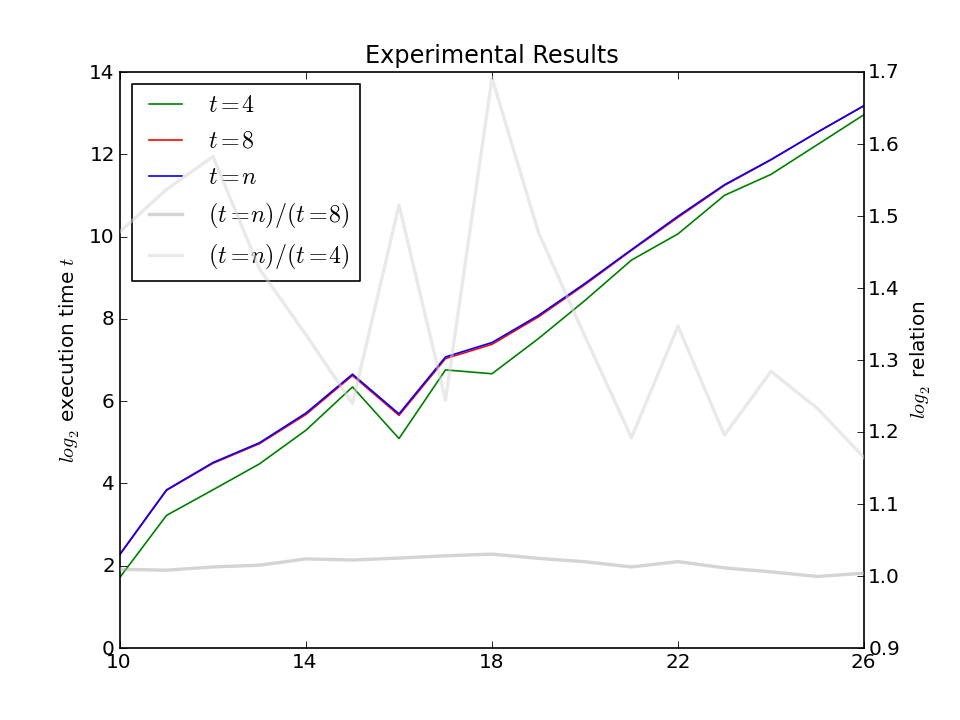
\includegraphics[width=0.7\textwidth,keepaspectratio=true]{experiments.png}
 \caption{Experimental verification for $t \in \{4,8,n\}$ with $m=\lfloor 0.1 n^2\rfloor$.}
 \label{fig:experiments}
\end{figure}

We note that in Table~\ref{table-eqnsolving} for $m = n \log n$ the complexity appears to grow sub-exponentially in $n$, which matches the behaviour over $\Z_2$ for which explicit formulas exist in literature \cite{Bardet}. Thus, we conclude that the statement in \cite{CCGHC10} that the scheme is secure against collusion attacks involving $m \approx 0.1n^2$ identities is incorrect. In particular, we expect sub-exponential complexity for $m \approx n \log n$. Furthermore, Figure~\ref{fig:experiments} disproves the claim made in \cite{susilo-baek:asiaccs2011} that Gröbner basis techniques cannot solve systems of equations in more than 15 variables.

\section{Refining the Basic Attack}\label{sec-attacks}

We now extend the basic collusion attack shown in Section \ref{sec-scheme},
exploiting the fact that the adversary can precompute the hash function $H_0$
in an effort to find identities leading to simpler sets of equations in the $n$
unknowns $x_i$. Our main idea is to partition the set of unknowns into subsets
of equal size, and
then search for identities yielding systems of equations with unknowns
restricted to these sets. Since the subsets are of
smaller size than the whole, solving these systems should be easier than solving
a single large system.

To this end, we write $n=2^d$, assuming this parameter is an integer power of 2
(as it is for the
concrete parameters in \cite{CCGHC10}). For some value $s \ge 0$ with $2^{d-s} \ge t$,
we partition the set $\{0,\ldots,n-1\}$ into $2^{s}$ sets $S_i$ each containing
$2^{d-s}$ integers by setting
$S_i=\{i2^{d-s},\ldots,(i+1)2^{d-s}-1 \}$. Next we present pseudo-code for our
attack.

\begin{algorithmic}
\STATE \hfill \\
\STATE Set $ID_i :=\emptyset, c_i :=0$ for $0\le i <2^s$
\STATE Set $c:=0$ and $c_{2^s}:=0$.
\REPEAT
    \STATE $c:=c+1$
    \STATE $id \leftarrow_R \{0,1\}^*$
    \IF {$H_0(id) \subset S_i$ for some $i$}
        \STATE $ID_i=ID_i \cup id$
        \STATE $c_i:=c_i+1$
    \ELSE
        \STATE $c_{2^s}:=c_{2^s}+1$
    \ENDIF
\UNTIL $c_i \ge m$ for $0 \le i <2^s$
\STATE Obtain $x_{id}$ for the first $m$ elements in each set $ID_i$ using key
extraction queries.
\FOR {$0 \le i < 2^s$}
    \STATE Using the $m$ values $x_{id}$ for $id \in ID_i$, generate and solve a
system of $m$ equations in the set of unknowns $\{ x_j: j \in S_i \}$.
\ENDFOR
\end{algorithmic}

The attack involves three main stages: a pre-computation to generate sets of
identities $ID_i$ suitable for building systems of equations; making key
extraction queries to obtain the required private keys; generating and solving
$2^s$ systems of equations, each containing $m$ equations in $2^{d-s}$
unknowns. Here $s$ and $m$ are parameters of our attack. It is evident that our
attack requires $m2^s$ key extraction queries, and that Table
\ref{table-eqnsolving} can be used to estimate the running time of the equation
solving stage for parameters of interest. We focus next on the running time of
the first stage.

The first stage involves making sufficiently many queries to $H_0$ so as to
obtain at least $m$ identities $id$ in each of the $2^s$ sets $ID_i$. In
practice, the identities $id$ will be drawn from the set of strings of some
maximum length. This makes no difference to the attack provided that $H_0$ acts
as a random function from $\{0,1\}^*$ to $t$-subsets of $\{0,1,\ldots,n-1\}$.
We make this assumption henceforth. Under this assumption, for a uniformly
selected $id$, the probability that $H_0(id) \subset S_i$ is equal to
$p:={2^{d-s} \choose t} /{n \choose t}$.

After $c$ iterations of main loop in the algorithm, the vector
$(c_0,\ldots,c_{2^s-1},c_{2^s})$ follows a multinomial distribution with
parameters $c$ and $(p,\ldots,p,1-2^sp)$. It then follows from standard results
on the multinomial distribution that, for each $0 \le i <2^s$, the random
variable $c_i$ follows a binomial distribution with mean $cp$ and variance
$cp(1-p)$. Moreover, the covariance between $c_i$ and $c_j$ is equal to
$-cp^2$. Since $p$ is generally small for the parameters of interest, the
covariance is very small and to a first approximation we may treat the first
$2^s$ values $c_i$ as independent identically distributed random variables. We
require each of these variables to be greater than $m$ for the algorithm to
terminate, and we estimate the probability that it does so after no more than
$c$ iterations as follows.

Using known estimates for the tail of the binomial distribution (see for
example \cite[Theorem A.13]{AS}), we have, for any real number $a$:
\[
\Pr[c_i \ge cp-a] > 1 - e^{-a^2/2pc}
\]
Under our assumption that the $c_i$ may be treated as independent random
variables, we then have:
\[
\Pr[\bigwedge_{0 \le i < 2^s}c_i \ge cp-a] > (1 - e^{-a^2/2pc})^{2^s}.
\]
Setting $a=m$ and $c=2m/p$, we then obtain:
\[
\Pr[\bigwedge_{0 \le i < 2^s}c_i \ge m] > (1 - e^{-m/4p})^{2^s} \ge
1-2^se^{-m/4p}\ge
1-\frac{n}{t}e^{-m/4p}.
\]
It is then easy to see that with $p = {2^{d-s} \choose t} /{n \choose t}$, the
algorithm terminates with high probability provided the main loop is executed
$c=2m/p$ times.

\paragraph{A concrete example:} We take $n=512$ (so $d=9$) and $t=8$, as in the concrete parameters suggested in \cite{CCGHC10}. We then select $s=4$ and $m=0.5 (2^{d-s})^2=2^{9}$ (corresponding to the last column in Table \ref{table-eqnsolving}). For these parameters, we have $p=2^{-33.3}$. Then our attack requires $2m/p=2^{43.3}$ evaluations of $H_0$ and $m2^s=2^{13}$ key extraction queries to build $2^s=16$ sets of $2^{9}$ equations in 32 variables. From Table \ref{table-eqnsolving}, the complexity of solving the 16 systems of equations is $16 \times 2^{26} = 2^{30}$ field operations. To summarise, we can break the scheme of \cite{CCGHC10} for the concrete parameters $n=512$ and $t=8$ using $2^{43.3}$ evaluations of $H_0$, $2^{13}$ key extraction queries and $2^{30}$ field operations. We remind the reader that our attack recovers the master secret key of the scheme, so our break is a complete one. We also remind the reader that the authors of \cite{CCGHC10} suggest that their scheme should be secure provided the attacker is limited to making no more than $0.1 n^2$ key extraction queries. Here, this equates to $2^{14.68}$ queries, while our attack needs only $2^{13}$ queries.

\paragraph{A second example (minimising key extractions):} We take $n=512$ (so $d=9$) and $t=8$, again as in the concrete parameters suggested in \cite{CCGHC10}. We then select $s=6$ and $m=9$. Then our attack requires $2^{60.8}$ evaluations of $H_0$, just $2^{9.2}$ key extraction queries and $2^{27.2}$ field operations to recover the master secret key of the scheme.

\paragraph{A third example (doubling the parameters):} Suppose the scheme parameters are doubled in an attempt to avoid our attack. So we take $n=1024$ (so $d=10$) and $t=16$. We then select $s=3$ and $m=2^{13}$. Our attack then requires $2^{64.1}$ evaluations of $H_0$, $2^{16}$ key extraction queries and $2^{41}$ field operations.

\paragraph{Further refinements of the attacks:}
We have taken a simple approach to generating sets of equations that are easier to solve than sets involving all $n$ variables. The reader can easily see that more sophisticated ways of generating and solving sets of equations can be developed. For example, once the values of some variables are known, we can be less restrictive about how further sets of equations are generated. However, this seems unnecessary in order to conclude that the scheme of \cite{CCGHC10} is flawed in an essential way.

\section{Conclusions}
We have presented an analysis of a recently proposed IBE scheme of Chen {\em et al.} \cite{CCGHC10}. We have shown that the main security result in \cite{CCGHC10} does not hold, and that the authors' assessment of their scheme's resistance to collusion attacks is over-optimistic. We have shown how standard Gr\"{o}bner basis techniques can be used to efficiently break the scheme for the parameters proposed in \cite{CCGHC10}, using a collusion attack with a small number of key extraction queries. Our attack is still practical if all the scheme's parameters are doubled.

We note that in order to achieve $80$-bit security against the simple attack from Section 2 one needs at least $n=2^{14}$. In that case, solving the system of equations would cost $n^6 = 2^{14\cdot6} = 2^{84}$ finite field operations. With such parameters the master public key $mpk$ would have a size of $160 \cdot 2^{14} / 8$ = 320kb. Note that this variant would still be vulnerable to the attacks in Section 4. For example, if we were to pick $s=4$, we would need $2^{52.04}$ evaluations of $H_0$, $2^{23}$ key extraction queries and just $2^{31}$ field operations in the Gr\"{o}bner basis step.

We conclude that the scheme of \cite{CCGHC10} does not offer an attractive trade-off between security and efficiency.

\begin{thebibliography}{10}
\bibitem{AS} N.~Alon and J.H.~Spencer. The probabilistic method. John Wiley \& Sons, 1992.

\bibitem{ars-faugere:asiacrypt04} G.~Ars, J.-C.~Faug\`ere, H.~Imai, M.~Kawazoe and M.~Sugita. Comparison between {XL} and {G}r\"obner basis algorithms. In \emph{Advances in Cryptology - ASIACRYPT 2004}, Volume 3329 of LNCS, pp. 338-353, Springer Verlag, 2004.

\bibitem{Bardet} M.~Bardet, J.~Faug\`{e}re and B.~Salvy. On the complexity of Gr\"{o}bner basis computation of semi-regular overdetermined algebraic equations. In \emph{Proceedings of the International Conference on Polynomial System Solving}, pp. 71-74, 2004.

\bibitem{Magma} W.~Bosma, J.~Cannon and C.~Playoust, {The {MAGMA} {A}lgebra {S}ystem {I}: {T}he {U}ser {L}anguage}. In \emph{Journal of Symbolic Computation}, Vol. 24, pp. 235-265. Academic Press, 1997.

\bibitem{CCGHC10} Y.~Chen, M.~Charlemagne, Z.~Guan, J.~Hu and Z.~Chen. Identity-based encryption based on DHIES. In D.~Feng, D.A.~Basin and P.~Liu \emph{Proceedings of the 5th ACM Symposium on Information, Computer and Communications Security, ASIACCS 2010}, pp. 82-88, ACM, 2010.

\bibitem{Cox} D.~Cox, J.~Little and D.~O'Shea. \emph{Ideals, Varieties, and Algorithms}. 3rd Ed. Springer Verlag. Berlin, Heidelberg, New York, 2007.

\bibitem{F4} J.-C.~Faug\`{e}re. A New Efficient Algorithm for Computing {G}r{\"o}bner Bases ({F4}). In \emph{Journal of Pure and Applied Algebra}, Vol.
139 (1-3), pp. 61-88, 1999.

\bibitem{F5} J.-C.~Faug\`{e}re. A New Efficient Algorithm for Computing {G}r{\"o}bner Bases without Reduction to Zero ({F5}). In \emph{Proceedings of the 2002 International Symposium on Symbolic and Algebraic Computation}, pp.75-83, ACM, 2002.

\bibitem{lazard:eurocal83} D.~Lazard. Gr\"obner-Bases, {G}aussian elimination and resolution of systems of algebraic equations. In \emph{Proceedings of the European Computer Algebra Conference on Computer Algebra}, Vol. 162 of LNCS, pp. 146-156, Springer Verlag, Berlin, 1983.

\bibitem{susilo-baek:asiaccs2011} W.~Susilo and J.~Baek. On the Security of the Identity-based Encryption based on {DHIES} from {ASIACCS 2010} (short paper). In \emph{Proceedings of the 6th ACM Symposium on Information, Computer and Communications Security, ASIACCS 2011}, ACM, 2011, to appear.

\bibitem{Sage} W.~Stein \emph{et al.} Sage Mathematics Software. Version 4.6.0. 2010
\end{thebibliography}

\end{document}


